\documentclass[11pt, letterpaper, twoside]{article}
\usepackage[utf8]{inputenc}
\usepackage[T1]{fontenc}
\usepackage{fancyhdr}
\usepackage[margin=1in, include foot]{geometry}
\usepackage{ragged2e}
\usepackage[]{hyperref}
\usepackage{apacite}
\usepackage{setspace}
\usepackage{caption}
\usepackage{subcaption}
\usepackage{etoolbox}
\usepackage{graphicx}
\usepackage{amsmath, amssymb}
\usepackage{cleveref}
\usepackage{wrapfig}
\usepackage{afterpage}
\usepackage{floatrow}
\usepackage{tikz}
\usepackage{booktabs}
\usepackage{siunitx}
\usepackage{dcolumn}
\usepackage{pdflscape}
\usepackage{adjustbox}
\usepackage{tablefootnote}
\usepackage{multicol}
% \usepackage{showframe}


\setlength{\parindent}{0pt}
\floatsetup[table]{capposition=top}

\title{\singlespacing\textbf{The Capture of Academic Economists}}


\author{
    Luigi Zingales\thanks{Booth School of Business, University of Chiacgo} \\
    \and
    Tommaso Valletti\thanks{Imperial College London}\\
    \and
    John Barios\thanks{Olin Business School, Washington Universty in St. Louis}\\
    \and
    Filippo Lancieri\thanks{Center on Regulation in Europe, ETH Zurich} \\
    \and
    Aditya Pollisety\thanks{Imperial College London}\\
    \and
    Joshua Levy \thanks{Booth School of Business, University of Chicago}\\
    \and
    Jonathan Lee \thanks{Carnegie Mellon University}
    }

\date{\today}

\onehalfspacing
\begin{document}
\begin{titlepage}   
    \maketitle
    \thispagestyle{empty}
\end{titlepage}


\newpage
\pagenumbering{arabic}

\section{Introduction}
Academic economists regularly serve as experts in a number of policy debates. In particular, they play an outsized role in the application of antitrust law, often serving as consultants to firms as well as the government through the guideline-setting, merger, and litigation processes. Because they are often relied upon to serve as experts and because of the broad social-welfare effects of antitrust enforcement (or lack thereof), the capture of academic industrial organization economists stands to be especially pernicious.\\

In many cases, senior economists with experience in the field serve as ``consultants'' to large firms which are, in turn, retained by legal counsel in the course of the mergers and acquisitions process. Consultants may help firms prepare for their merger filings and, if those applications are challenged by the government, may serve as ``expert witnesses'' in the course of ensuing litigation. The expert witness role of being a consultant is what makes academic economists potentially open to capture. Take, for example, an economist whose academic research (agenda) may run counter to the interests of the firms they represent. If such research were to be published in academic journals (which are readily available to the interested public), counter-party litigators may find that work and use it undermine the consultant's credibility or reputation as an expert during cross-examination, all to the detriment of the economist's clients. Consequently, consulting economists, not wanting to lose their well-remunerated positions as expert witnesses, may engage in self-censorship with respect to certain contentious topics that may be subject to litigation, or to be even more cautious, may abandon entire courses of research.\\

This poses a number of problems. First, capture of economists detracts from the stated enterprise of the academic community: the search for truth. Abandoning that search represents tacit intellectual dishonesty (even when a scholar is resource constrained) if not an outstanding form of corruption. Second --- though no-less important --- are the indirect effects of that intellectual dishonesty. If further research on the socio-political effects of antitrust-enforcement, per se, could be demonstrated to yield positive returns (by ways of advocating for preventing mergers or for breaking up large firms, for example), abandoning that research incurs an opportunity cost for society.\\

Economists who consult thus face a conflict of interests between their intellectual obligations to unbiased research and personal enrichment. We propose that the publishing behaviors of consultant academic economists (who have been captured by industry) differs systematically from their peers who do not engage in consulting. What follows is a description of the datasets that have been collected to date investigate this question.


\section{Papers Database}

We begin by collecting a database of academic papers in leading general-interest and field-specific journals. The jouranls of interest are noted below in Table 1. In addition to the ``Top 5'' general-interest journals, we begin collecting the corpus of articles published in prominent field journals in 1) industrial organization (IO) and law and economics; 2) financial economics; and 3) labor economics. We are primarily interested in the role of consulting firms in antitrust enforcement so the IO field can be thought of as a ``treatment'' group. The latter two fields serve, in effect, as a kind of weak control. Financial economists and labor economists also regularly engage various consulting activities. However, those relationships are of a different nature to those of IO economists who work in antitrust because they rarely take place in an adversarial (litigated) context. So, even though financial and labor economists may also face material conflicts of interest, they are not necessarily open to capture in the same way that IO economists are. 

\begin{table}[!h] \centering
    \caption{Journals in Sample}
    \label{}
\footnotesize
\begin{tabular}{@{\extracolsep{5pt}} llcc} 
\hline \\[-1.8ex] 
 & Title & Code & ISSN  \\ 
\hline \\[-1.8ex] 
\textsc{Top 5} & & \\
& American Economic Review & AER & 00028282\\
& Econometrica & ECA & 00129682\\
& Journal of Political Economy & JPE & 00223808\\
& Quarterly Journal of Economics & QJE & 00335533\\
& Review of Economic Studies & RES & 00346527\\
\textsc{IO \& Law and Econ} & & \\
& Antitrust Bulletin & ATB & 0003603X\\
& Antitrust Law Journal & ALJ & 00036056\\
& Journal of Economics and Management Strategy & JEM & 15309134\\
& Journal of Human Resources & JHR & 0022166X\\
& Journal of Law and Economics & JLE & 00222186\\
& Journal of Law, Economics, and Organization & JOL & 87566222\\
& RAND Journal of Economics & RJE & 07416261\\
\textsc{Finance} & & \\
& Journal of Finance & JOF & 00221082\\
& Journal of Financial Economics & JFE & 0304405X\\
& Review of Financial Studies & RFS & 08939454\\
\textsc{Labor} & & \\
& Journal of Labor Economics & JOL & 0734306X\\
\hline \\[-1.8ex]
\end{tabular}
\end{table}

\subsection{Sources}
We are interested in understanding the patterns of publishing behavior by consulting and non-consulting economists. So, we are primarily interested in article meta-data. We begin by turning to two different sources:

\subsubsection{Scopus}
Scopus is a bibliometric and citation service produced and maintained by Elsevier, a publishing company. Scopus is attractive as data source because it systematically covers many of the dimensions of interest. It contains paper-level and author-level meta-data. Most importantly, it generates a unique ``author ID'' for every author. This becomes the foreign key by which we can match individuals with a vast array of other data.

\subsubsection{EconLit}
EconLit is another bibliometric service maintained by EBSCOHost. In contrast to Scopus, which covers all disciplines and fields of study, EconLit covers exclusively Economics journals. Moreover, because EconLit is primarily focussed on papers as the unit of analysis, EBSCOHost does not engage in the same kind of standardization that Elsevier does. Consequently, the database is not as ``relational'' as Scopus is. An author who appears as ``L. Zingales'' in one journal article is not associated with the ``Luigi Zingales'' who appears in a different journal, even though they are the same person.\\

In contrast to Scopus however, the disciplinary focus of EconLit means that it carries ``Journal of Economic Literature (JEL) codes.'' JEL codes are alphanumeric codes chosen by article authors that describe the fields that a paper pertains to. For example, an author of a paper about vertical restraints might label her paper with ``L42'' the code that corresponds to ``Vertical Restraints; Resale Price Maintenance; and Quantity Discounts.'' Each character in a JEL code represents a certain degree of specificity: the first alphabetic character identifies the broadest relevant field, and the first and second numbers indicate increasingly specific sub-fields and topics.\\

The presence of JEL codes on EconLit-derived observations allows us to determine the focus of the article beyond what can be inferred from the title and publication, without having to read it in full. JEL codes additionally can be used to characterize how the literature changes in focus over time.\footnote{The \textit{Antitrust Law Journal} is not tracked by EconLit. So all data for that journal is derived only from Scopus.}

\subsection{Matching}

There is considerable intersection between the Scopus and EconLit databases. However, Scopus generally represents a subset of the articles that are present in EconLit.\footnote{The notable exception to this is the \textit{Journal of Financial Economics}} Additionally, there are minor inconsistencies (punctuation, capitalization, etc.) between the ways the two parties record various fields of interest: title, author names, volume and issue numbers, etc. In order to assemble as complete a database of papers as possible we apply a fuzzy matching algorithm. First, articles that can be matched using only a modified title (coerced to all upper-case to eliminate capitalization inconsistencies), page-range, and volume and issues numbers are matched accordingly. This first step constitutes the ``naive'' match. For most journals of interest the naive match captures over 80\% of observations.\\

Following the naive match, we construct a ``closeness'' score for every pair-wise combination of remaining, unmatched articles from Scopus and EconLit. This score includes an average of three different Levenshtein-distance metrics that measures the edit-distance (how different) between two strings; volume and issue numbers; and page ranges. After computing all pair-wise scores, a match is only identified both articles are symmetrically best. That is, a match is made if and only if an article (A) from Scopus has a best candidate-match with an article (B) from EconLit \textit{and} vice versa. This fuzzy-matching process usually reduces the remaining unmatched articles by 50\%. The results of this process, by journal, are presented in Table 2 and Figure 1\\


% Table created by stargazer v.5.2.3 by Marek Hlavac, Social Policy Institute. E-mail: marek.hlavac at gmail.com
% Date and time: Tue, Jul 26, 2022 - 9:30:30 PM
\begin{table}[h] \centering 
  \caption{Results of Scopus-EconLit Matching} 
  \label{} 
\begin{tabular}{@{\extracolsep{5pt}} llccccc} 
\\[-1.8ex]\hline 
\hline \\[-1.8ex] 
 & Journal & Naive matches & Fuzzy matches & Scopus only & EconLit only &  \textsc{\textbf{Total}} \\ 
\hline \\[-1.8ex] 
\textsc{Top 5} & & & & & & \\ 
 & AER & 4449 & 354 & 11 & 876 & 4803 \\ 
 & ECA & 1513 & 54 & 7 & 351 & 1567 \\ 
 & JPE & 1205 & 87 & 26 & 301 & 1292 \\ 
 & QJE & 1199 & 76 & 27 & 64 & 1275 \\ 
 & RES & 1311 & 100 & 31 & 100 & 1411 \\ 
\textsc{IO \& Law and Econ} & & & & & & \\ 
 & ATB & 547 & 132 & 53 & 217 & 679 \\ 
 & JEM & 606 & 101 & 32 & 253 & 707 \\ 
 & JHR & 799 & 142 & 35 & 207 & 941 \\ 
 & JLE & 600 & 124 & 5 & 162 & 724 \\ 
 & JLO & 665 & 49 & 3 & 53 & 714 \\ 
 & RJE & 1060 & 109 & 19 & 95 & 1169 \\ 
 & JFE & 2473 & 141 & 214 & 3 & 2614 \\ 
\textsc{Finance} & & & & & & \\ 
 & JOF & 2256 & 168 & 12 & 23 & 2424 \\ 
 & RFS & 1809 & 154 & 63 & 196 & 1963 \\ 
\textsc{Labor} & & & & & & \\ 
 & JOL & 719 & 95 & 42 & 234 & 814 \\ 
\hline \\[-1.8ex] 
\end{tabular} 
\end{table} 


\begin{figure}[h]
    \centering    
    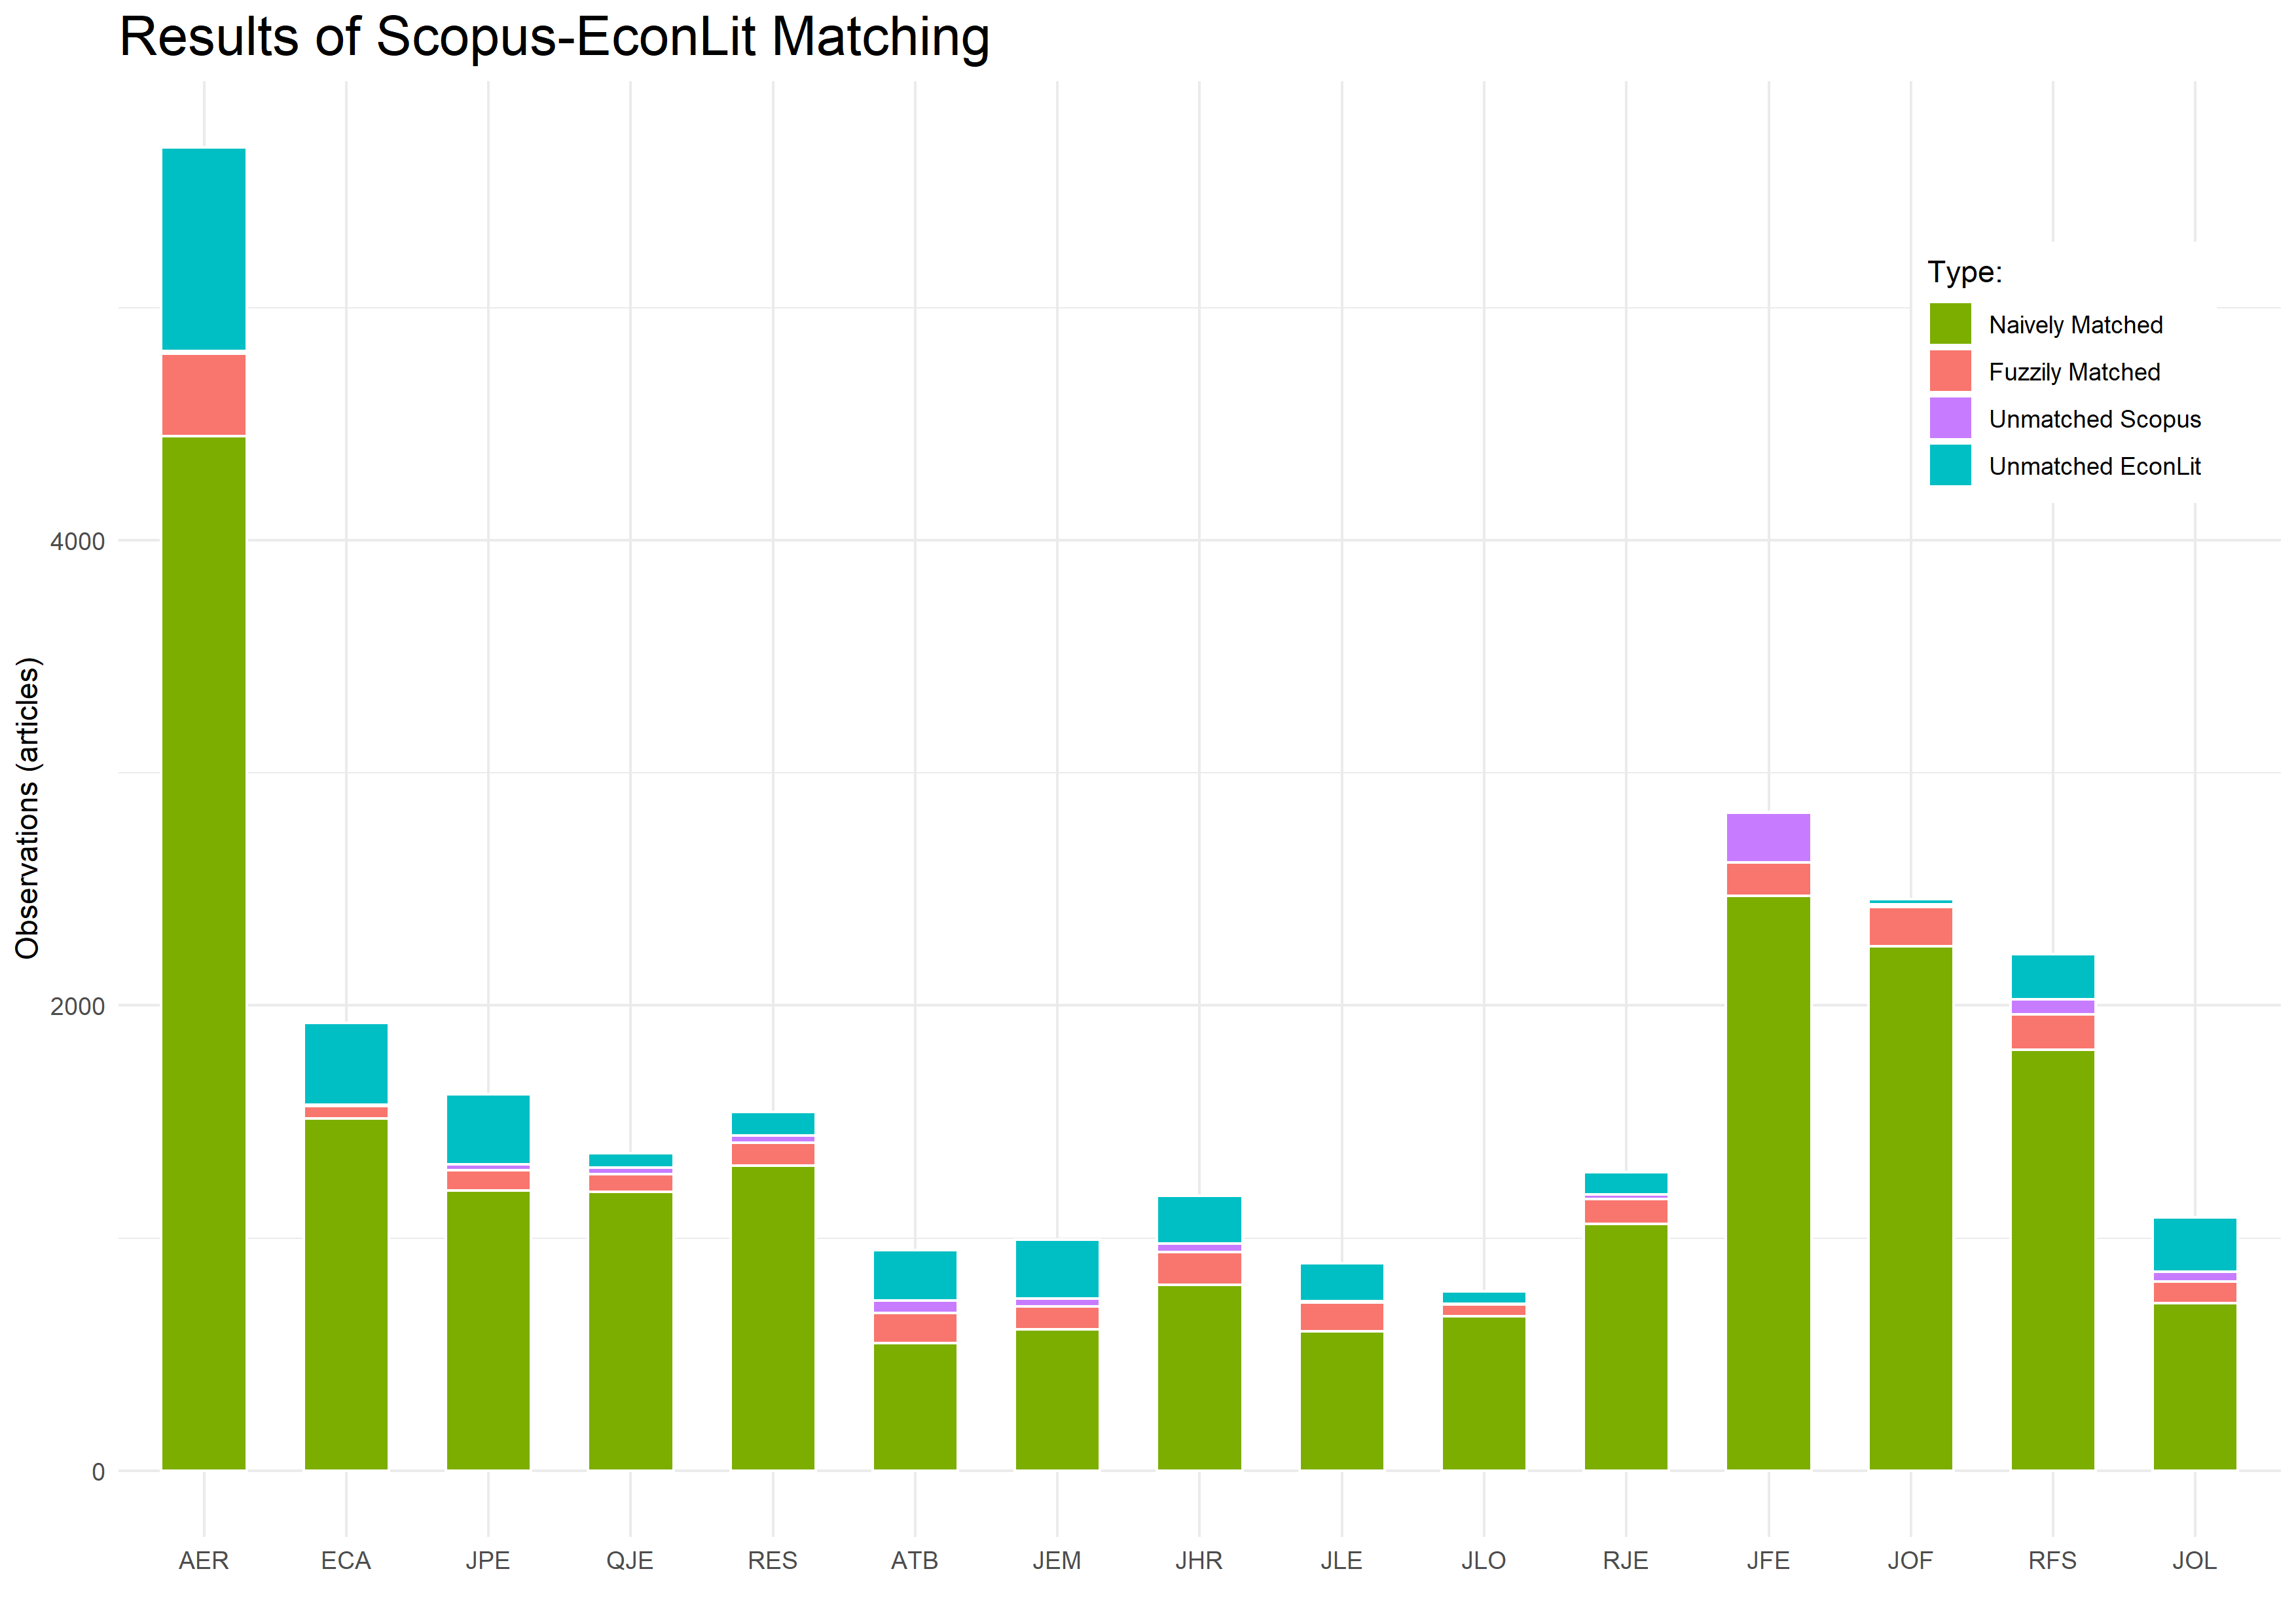
\includegraphics[width=\textwidth]{figures/scopus_econlit_matching_results.png}
    \caption{Results of the Scopus-EconLit Matching Process}
\end{figure}

Following this fuzzy matching process, some articles (mostly from) EconLit and Scopus remain unmatched. If necessary, we can choose to hand-match these remaining articles and/or keep them and attempt to infer additional variables of interest systematically or by hand. For example, we desire Scopus matches for EconLit observations because that allows us to identify the authors using the unique Scopus author ID. We desire the EconLit matches for Scopus observations because that provides us with JEL codes. It is possible to write an algorithm that tries to identify the best author-match in the Scopus database using the data already available in the EconLit database. Additionally, for the jouranls that provide them, it would be possible to collect JEL codes by hand.

\subsection{Results}
At present, we have over 24,000 unique paper observations from 16 journals over the period from 1990 to 2021. For most of these we have a ``balanced'' dataset that include the following variables:
\begin{multicols}{2}
    \begin{itemize}
        \item Author(s) (and unique identifier)
        \item Title (and unique identifier)
        \item Publication Name (and ISSN)
        \item Publication information (volume, issue, page-range, date)
        \item Abstract
        \item JEL codes (and descriptions)
    \end{itemize}
\end{multicols}

\subsection{Classifying Papers}
An outstanding challenge remains classifying the papers and their results. Doing this might be important because capture may be asymmetric. That is, consulting economists might censor particular \textit{kinds} of results because of the ramifications those results might have for their clients. For example, the professional sanction for writing a paper that finds consumer welfare benefits to market concentration might be considerably smaller (or non-existent) relative to writing a paper that finds that the same market concentration generates non-priced harms to consumers. This would lead to a bias in publication behavior that we have not yet developed a method for identifying.

\section{Scholars \& Consultants Database}
In addition to understanding the state of the literature (the response variable), we have built an early-stage dataset of authors and consultants (the explanatory variable). 

\subsection{Scholars}
Starting with all of the papers from the journal of interest collected from Scopus, we collect all of the associated authors. This is facilitated in large part because Scopus generates a unique author ID for each scholar. This facilitates joining papers to editors, placing scholars in co-authorship networks, and identifying consultants. As a possible extension of this dataset, we can use Scopus Author API to collect affiliation data for each scholar.\footnote{However, based on casual inspection, this appears to be inaccurate or not up to date.}

\subsection{Consultants}
We are particularly interested in the subset of scholars who are consultants --- and particularly those who serve as expert witnesses in antitrust litigation. However, selection and measurement bias are likely to play an outsized role in identifying consultants. We address each of these in turn.\\

First we attempt to handle selection bias by developing a database on the basis of a characteristic that we think should be exogenous to consulting engagements. For this, we begin by identifying all scholars affiliated with at least one of a number of research programs with the National Bureau of Economic Research (NBER). Using the same justificationas we did for journal selection (``treatments'' and ``controls''), we identify all scholars affiliated with the Industrial Organization, Law and Economics, Corporate Finance, and Labor Studies programs.\\

We then investigate each scholar to determine whether they are a consultant (or engage in consulting). There are four test we apply:
\begin{enumerate}
    \item We check the websites of major consulting firms, to see if the scholar of interest appears as a (active) consultant.\footnote{We consider Analysis Group, Bates White, Berkeley Research Group, the Brattle Group, Compass Lexecon, Charles River Associates, Cornerstone Research, Keystone, NERA, and Vega Economics as major firms for this step}. 
    \item We identify the scholar's personal website and CV and determine whether it lists any consulting engagements. 
    \item We construct a common Google search, ``[Scholar Name] expert witness/consulting'', and examine the first three pages of results to determine whether these results reveal any consulting engagements.
    \item We read the disclosure statements made by these scholars in their NBER working papers to identify any consulting relationships/conflicts of interest.
\end{enumerate}
Deviations from this procedure are noted in the database. In addition to noting whether a scholar engages in consulting with a consulting firm, we also note if the scholar of interest has engaged in any consulting, paid work for, or data-sharing agreements with private firms.\\

The challenge of measurement bias is also pertinent. Our methodology for identifying consultants is far from exhaustive and suffers from non-response problem. At present, there is not way segregate ``true negatives'' scholars who, in reality, do not consult from ``false negative'' scholars who do consult but do so sufficiently surreptitiously to evade our search methodology. This is an open challenge that could be resolved by gaining access to corporate or government/regulator data.

\subsubsection{Disclosure}
In addition to identifying whether a scholar consults, we also identify how and whether those scholars proactively disclose their potential conflicts of interest. To begin, we construct a naive index of transparency with scores of 0 being the most opaque and scores of 2 being the most transparency. A scholar's score increases by 1 point for disclosing conflicts of interest in their CV/website and/or their NBER working papers.\footnote{A scholar is coded as having declared their conflict of interest in their working papers if \textit{any} of their working papers disclose a conflict of interest.}. The results of this effort are presented in in Figures 2 (a) and (b).

\begin{figure}[h]
    \centering
    \begin{subfigure}[h]{0.45\textwidth}
        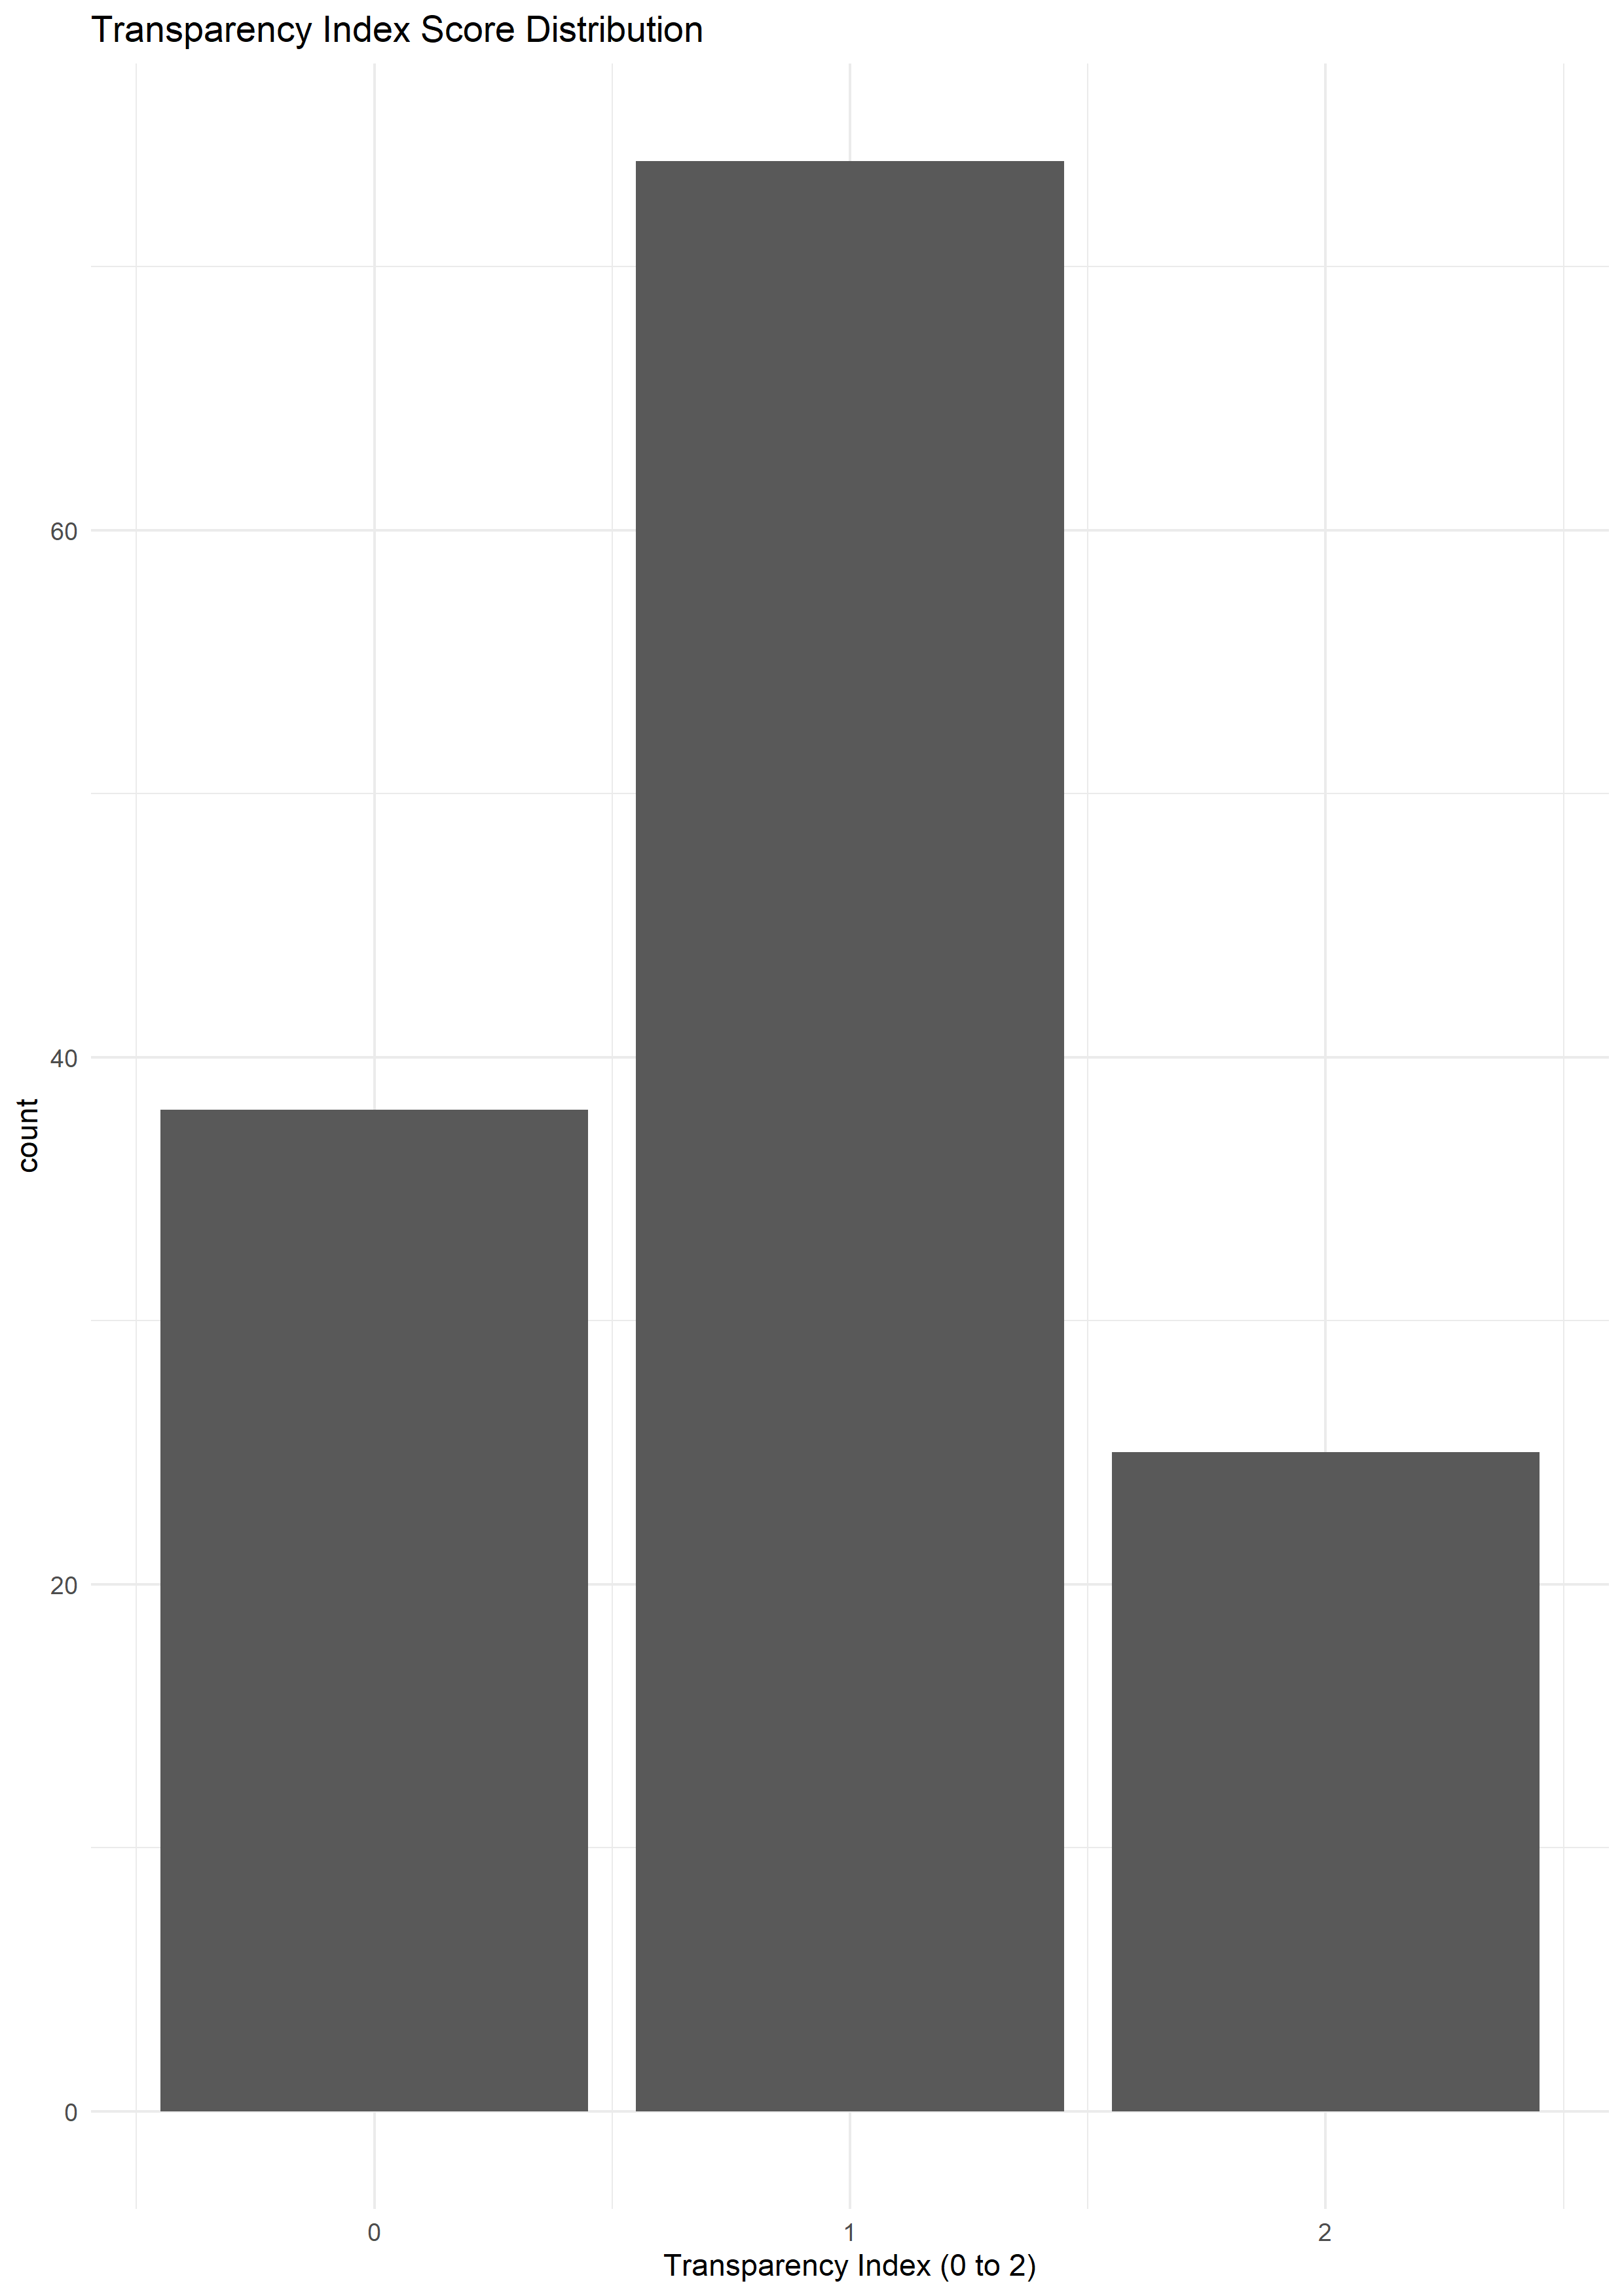
\includegraphics[width=\textwidth]{figures/transparencyPlot.png}
        \caption{All consultants}        
    \end{subfigure}
    \hfill
    \begin{subfigure}[h]{0.45\textwidth}
        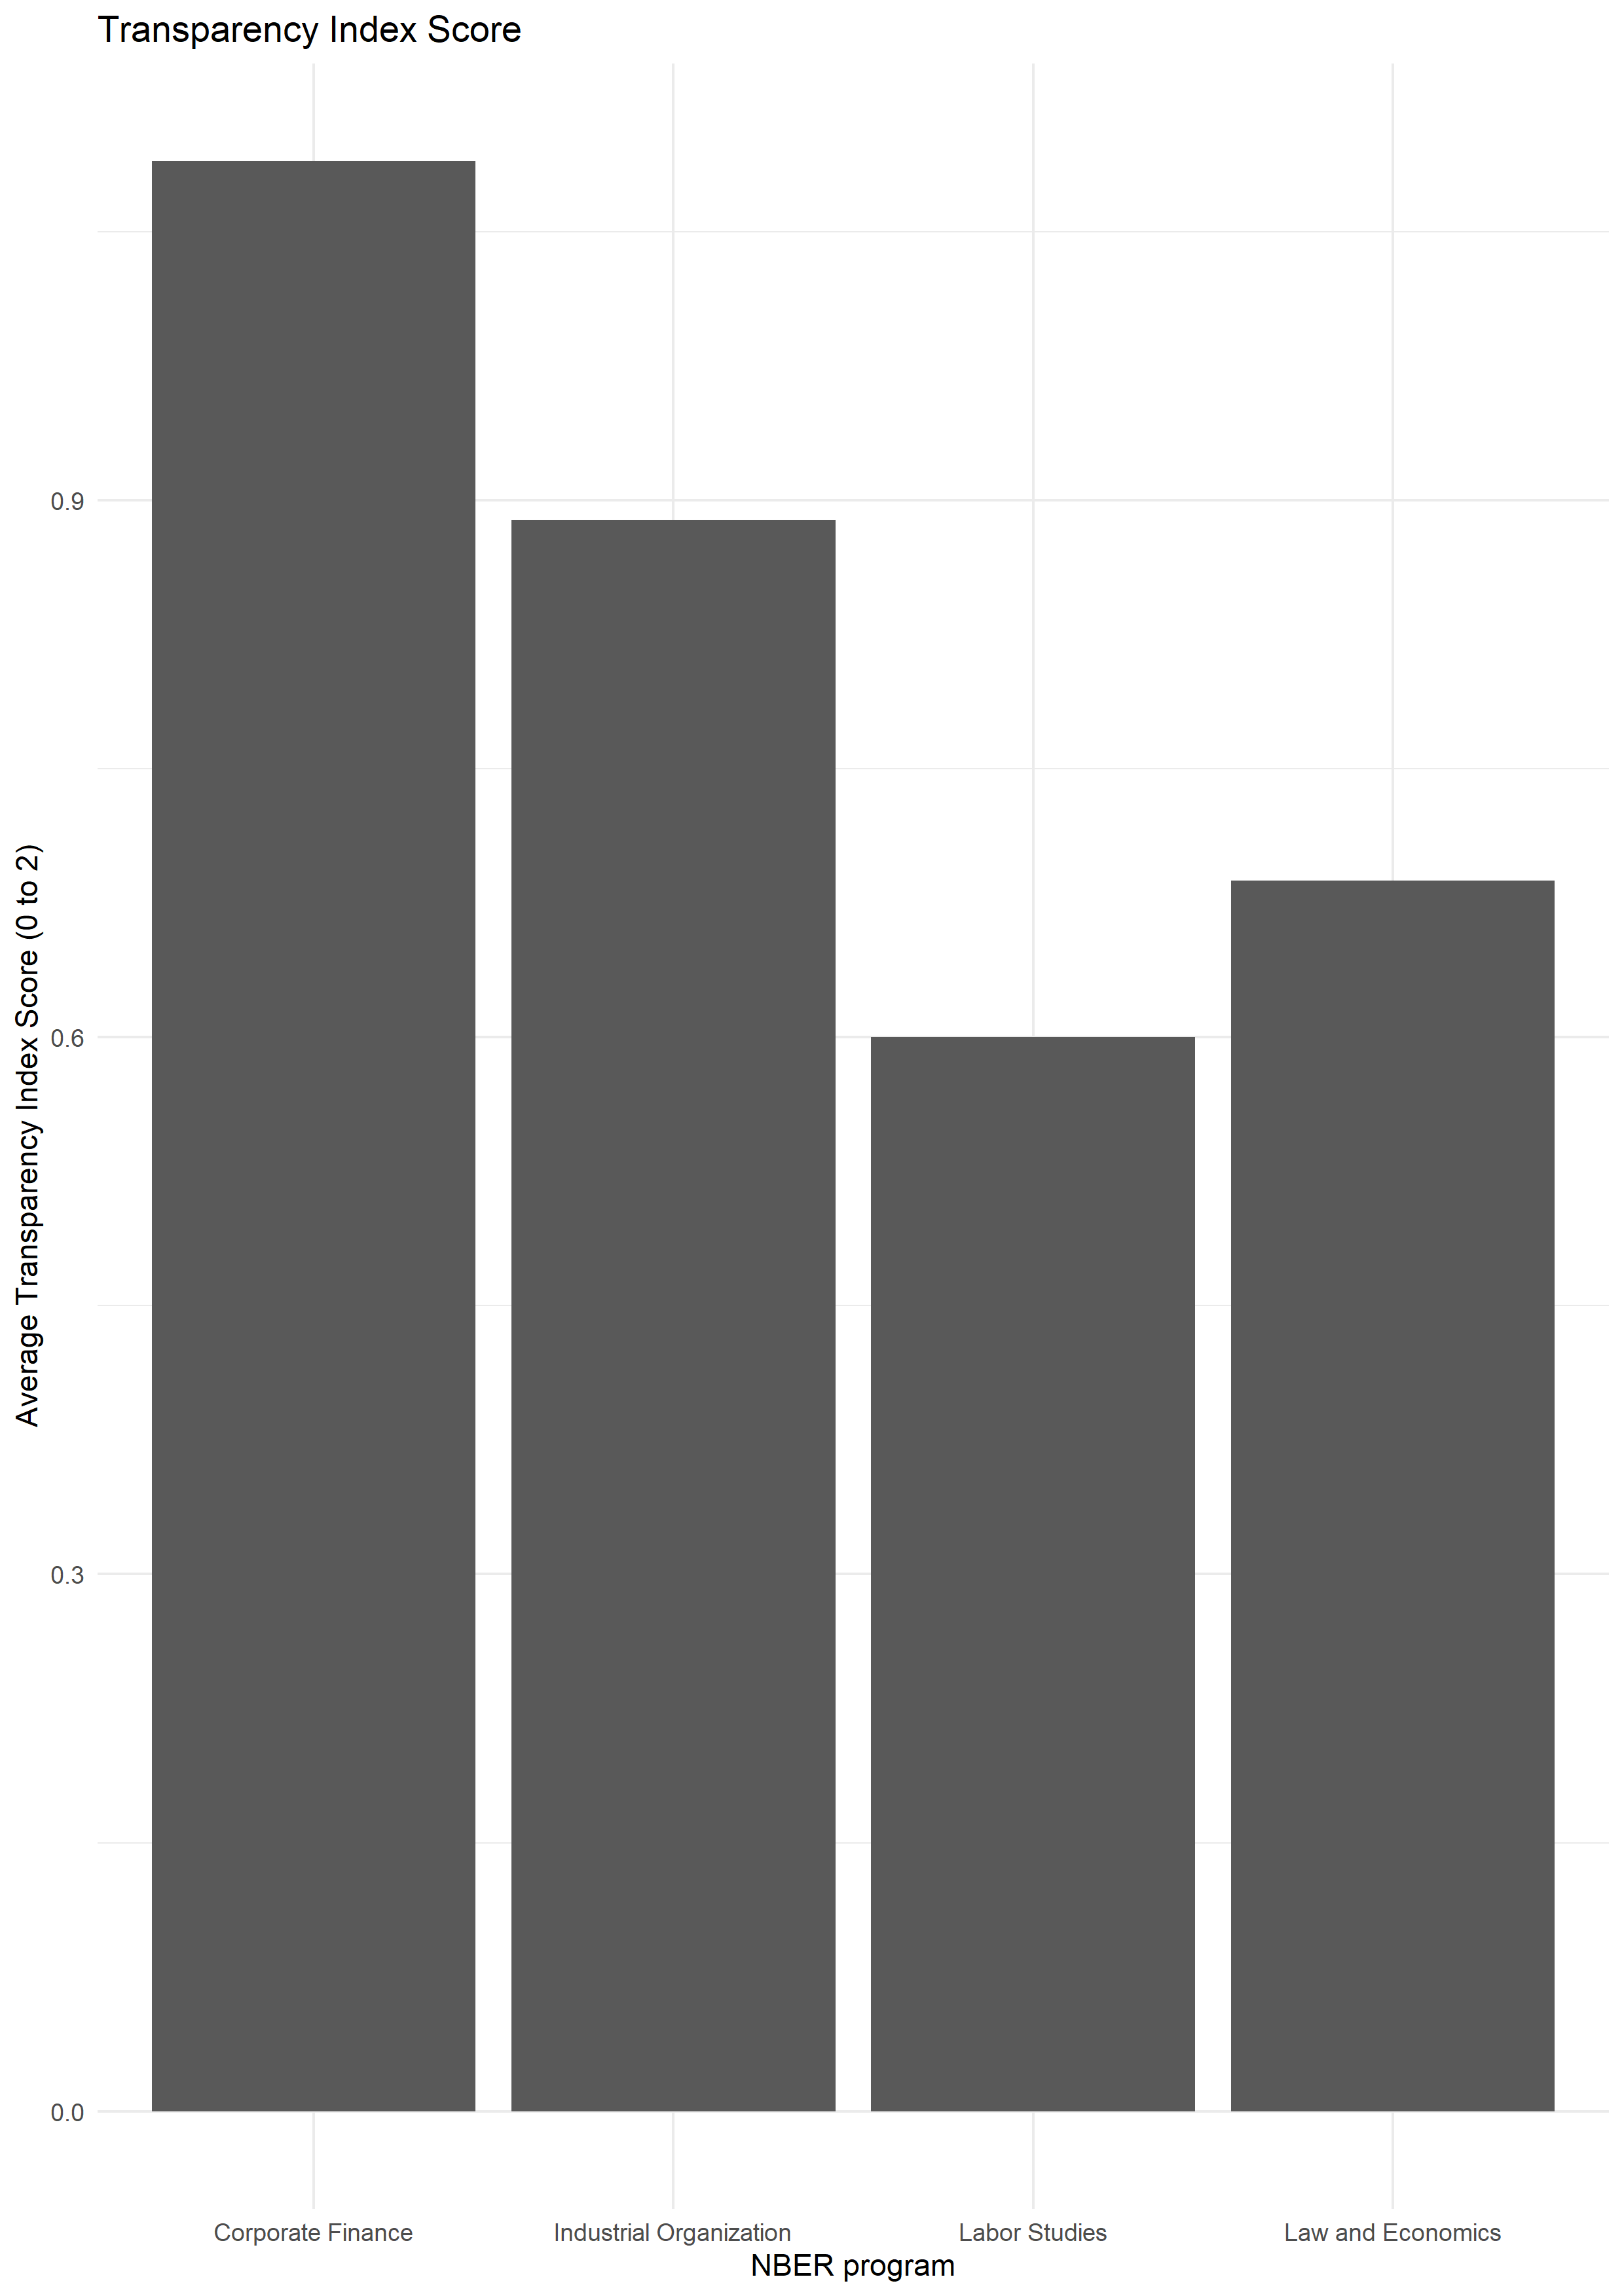
\includegraphics[width=\textwidth]{figures/transparencyByProgram.png}
        \caption{By NBER Program}
    \end{subfigure}
    \caption{Disclosure Transparency Index}
\end{figure}


% Table created by stargazer v.5.2.3 by Marek Hlavac, Social Policy Institute. E-mail: marek.hlavac at gmail.com
% Date and time: Wed, Jul 27, 2022 - 4:52:27 PM
\begin{table}[!htbp] \centering 
  \caption{Most Published Authors (all journals)} 
  \label{} 
\begin{tabular}{@{\extracolsep{5pt}} ccc} 
\\[-1.8ex]\hline 
\hline \\[-1.8ex] 
Name & Articles & Rank \\ 
\hline \\[-1.8ex] 
Andrei ShleiferNA & 89 & 1 \\ 
Daron AcemogluNA & 85 & 2 \\ 
Rene M. Stulz\textbackslash mathsection & 71 & 3 \\ 
Jean TiroleNA & 71 & 3 \\ 
Josh Lerner\textbackslash mathsection & 55 & 4 \\ 
James J. HeckmanNA & 53 & 5 \\ 
Jeremy C. Stein\textbackslash mathsection & 46 & 6 \\ 
John A. ListNA & 46 & 6 \\ 
Sheridan Titman\textbackslash mathsection & 44 & 7 \\ 
John J. SiegfriedNA & 44 & 7 \\ 
Raghuram RajanNA & 44 & 7 \\ 
\hline \\[-1.8ex] 
\end{tabular} 
\end{table} 


\subsubsection{Presence in Data}
As part of a descriptive exercise, we are additionally interested in understanding how consultants participate in the publishing process. First, using their unique Scopus IDs we match all NBER affiliated scholars to our papers database (described above). We then identify an article as being a consultant-article if at least one of the authors is a consultant. We identify an article as being NBER-affiliated if at least one of the authors is a member of an NBER research program (but not a consultant). The results of this exercise are plotted in Figure 3.\\

\begin{figure}[h]
    \centering    
    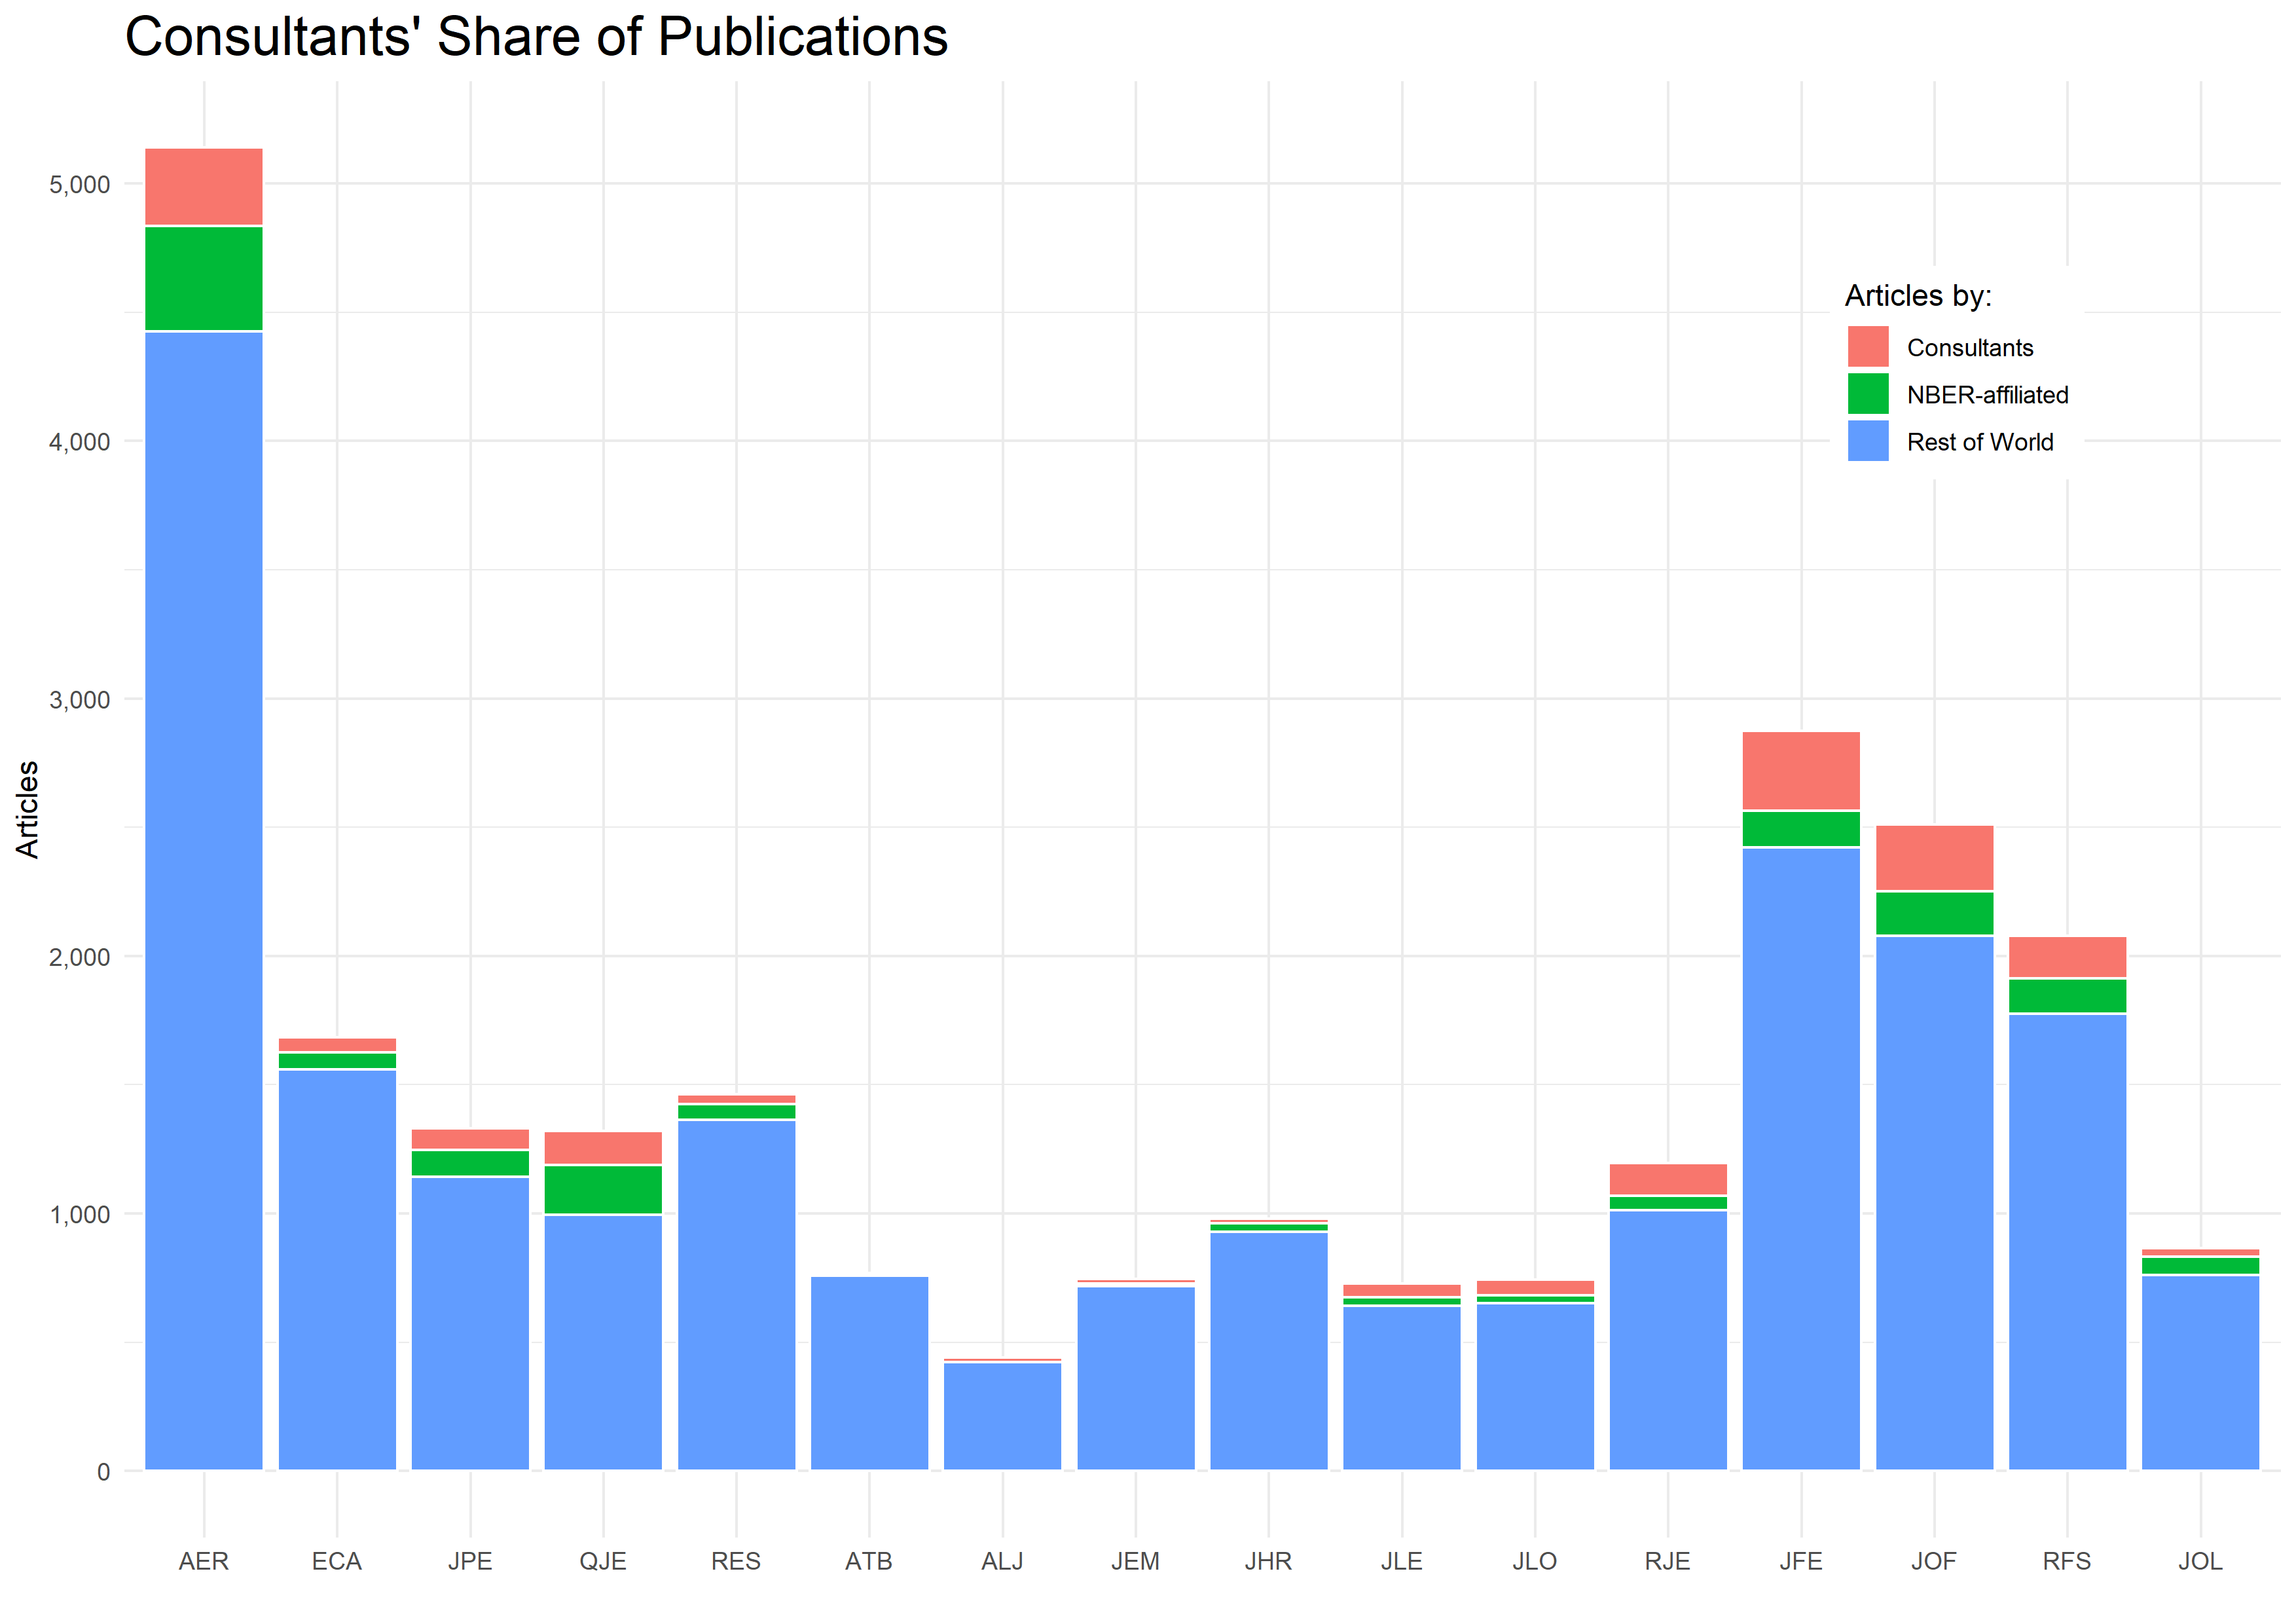
\includegraphics[width=\textwidth]{figures/consultants_nber_journal_share.png}
    \caption{Consultants' Share of Publications}
\end{figure}

A cursory inspection suggests that consultants and NBER do not dominate the journals of interest. However, consider that our papers database contains over 18,000 unique authors. In fact, considering that the 344 NBER scholars and consultants make up just under 2\% of the observed authors, these scholars are incredibly productive. This result is also borne out in Table 3, which identifies the most productive authors in our database.\footnote{Similar rankings are available by field and journal in Appendix A.} Those with super-scripted symbols are consultants and are affiliated with corresponding NBER program.Though not all are consultants, \textit{all} of the top 11 most productive scholars are affiliated with the NBER. Again, Table 4 depicts what is plotted in Figure, the extraordinary productivity of NBER members.\\





% Table created by stargazer v.5.2.3 by Marek Hlavac, Social Policy Institute. E-mail: marek.hlavac at gmail.com
% Date and time: Thu, Jul 28, 2022 - 5:38:20 AM
\begin{table}[!htbp] \centering 
  \caption{Consultants' Share of Publications} 
  \label{} 
\begin{adjustbox}{max width = \textwidth}
\begin{tabular}{@{\extracolsep{5pt}} llccccc} 
\\[-1.8ex]\hline 
\hline \\[-1.8ex] 
 & Journal & Count & Consultants (count) & Consultants (share) & NBER (count) & NBER (share) \\ 
\hline \\[-1.8ex] 
\textsc{Top 5} & & & & & & \\ 
 & American Economic Review & 5139 & 304 & 5.92\% & 410 & 7.98\% \\ 
 & Econometrica & 1684 & 57 & 3.38\% & 68 & 4.04\% \\ 
 & Journal of Political Economy & 1331 & 83 & 6.24\% & 106 & 7.96\% \\ 
 & Quarterly Journal of Economics & 1321 & 132 & 9.99\% & 193 & 14.61\% \\ 
 & Review of Economic Studies & 1462 & 36 & 2.46\% & 63 & 4.31\% \\ 
\textsc{IO \& Law and Econ} & & & & & & \\ 
 & Antitrust Bulletin & 770 & 11 & 1.43\% & 0 & 0.00\% \\ 
 & Antitrust Law Journal & 440 & 16 & 3.64\% & 0 & 0.00\% \\ 
 & Journal of Economics and Management Strategy & 746 & 18 & 2.41\% & 9 & 1.21\% \\ 
 & Journal of Human Resources & 980 & 17 & 1.73\% & 35 & 3.57\% \\ 
 & Journal of Law and Economics & 729 & 53 & 7.27\% & 34 & 4.66\% \\ 
 & Journal of Law, Economics, and Organization & 743 & 60 & 8.08\% & 31 & 4.17\% \\ 
 & RAND Journal of Economics & 1195 & 125 & 10.46\% & 56 & 4.69\% \\ 
\textsc{Finance} & & & & & & \\ 
 & Journal of Finance & 2510 & 259 & 10.32\% & 172 & 6.85\% \\ 
 & Journal of Financial Economics & 2873 & 310 & 10.79\% & 141 & 4.91\% \\ 
 & Review of Financial Studies & 2078 & 165 & 7.94\% & 138 & 6.64\% \\ 
\textsc{Labor} & & & & & & \\ 
 & Journal of Labor Economics & 865 & 32 & 3.70\% & 72 & 8.32\% \\ 
\hline \\[-1.8ex] 
\end{tabular} 
\end{adjustbox} 
\end{table} 



\section{Editors Database}
Also of interest is the role of editors in publishing. Editors have tacit powers to change the academic discourse by conditioning a paper's acceptance on certain changes, thereby emphasizing or understating certain conclusions. To begin investigating the role that editors play in attenuating or exacerbating academic capture, we begin creating a database of editors for each of our journals of interest.\footnote{This is still very much in progress.}. For each journal-calendar/volume-year we identify the composition of editorial staff, thereby allowing us to identify the tenure and position of each editor. To date, we have collected XXX unique editors. Below Figures 4, 5, and 6 plot the composition of editorial staff, the average tenure of editors, and the longest tenure of an editor, respectively, for a number of journals.\\

Figures 7 and 8 plot the history of editors at the \textit{Journal of Labor Economics} and \textit{Journal of Political Economy}, respectively.

\begin{figure}[h]
    \centering    
    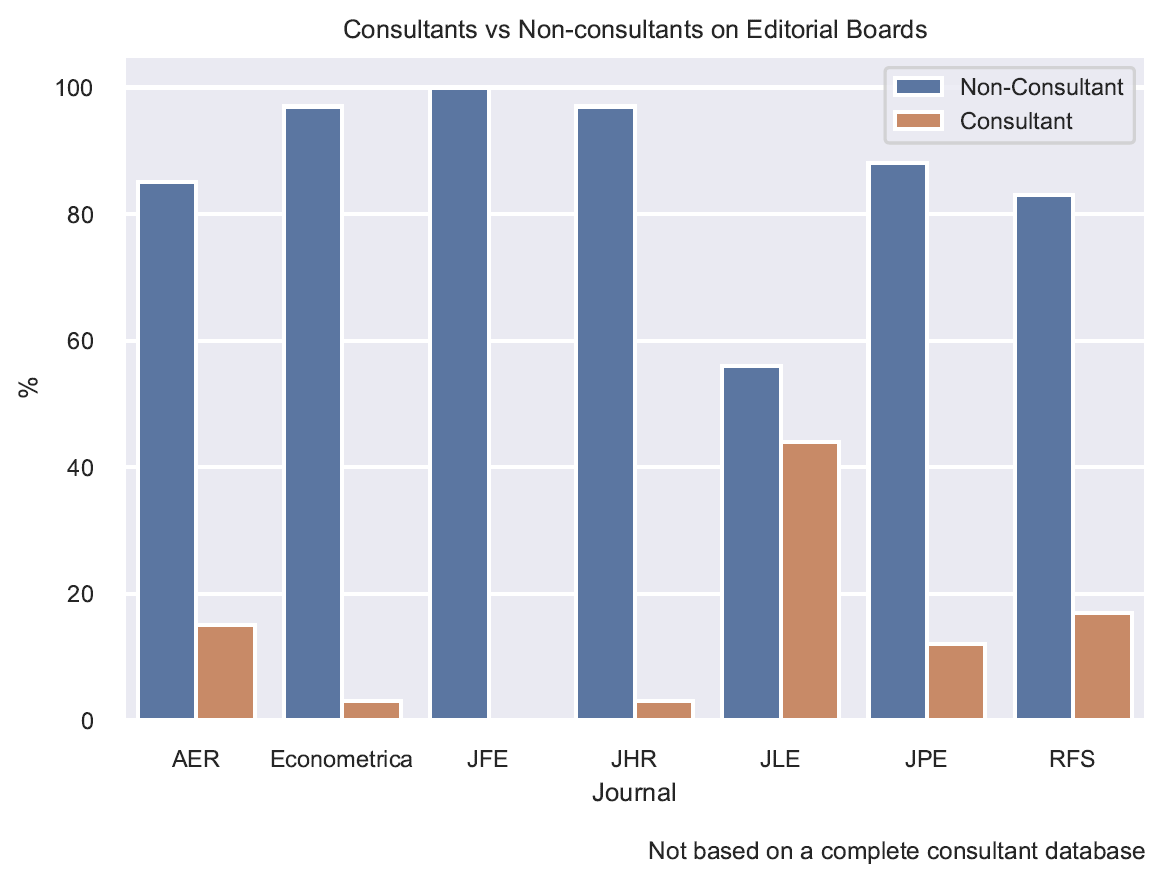
\includegraphics[width=\textwidth]{figures/total_editors.png}
    \caption{Results of the Scopus-EconLit Matching Process}
\end{figure}
\begin{figure}[h]
    \centering    
    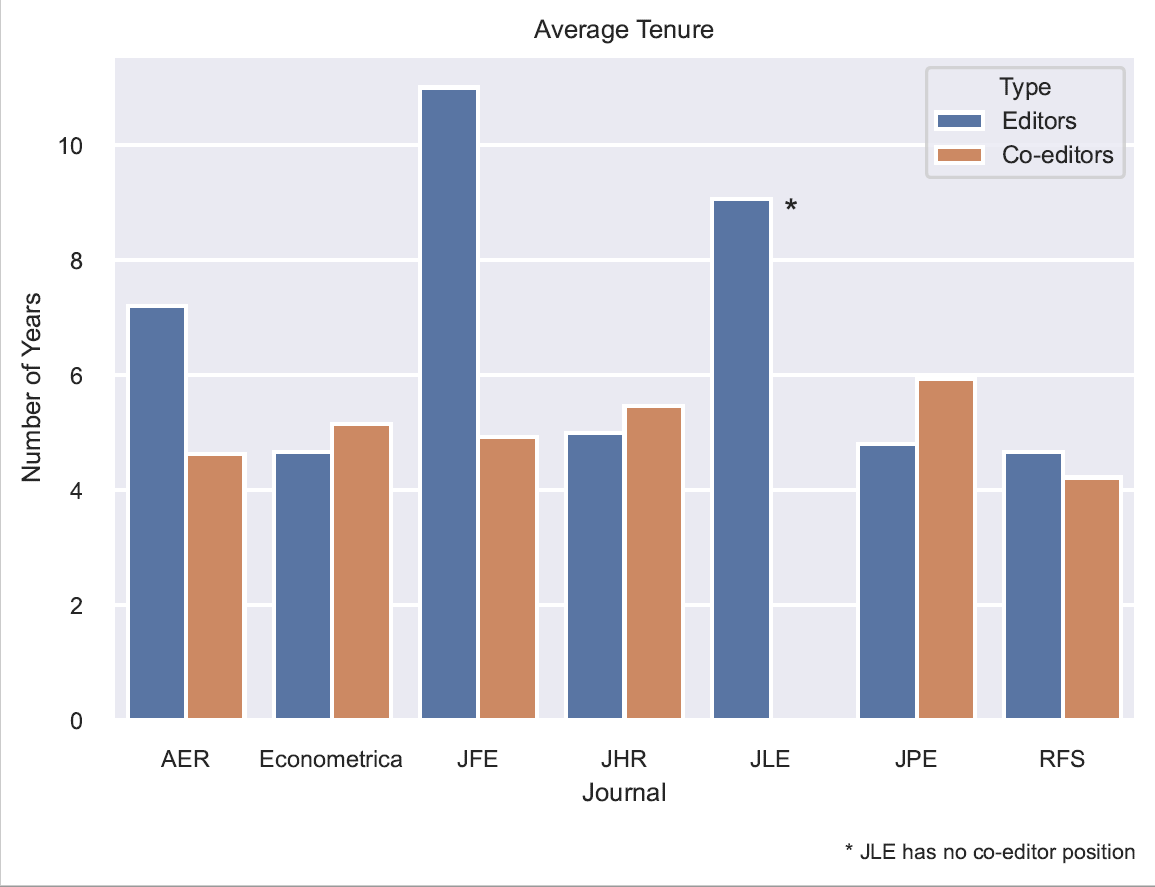
\includegraphics[width=\textwidth]{figures/editors_avg_tenure.png}
    \caption{Results of the Scopus-EconLit Matching Process}
\end{figure}
\begin{figure}[h]
    \centering    
    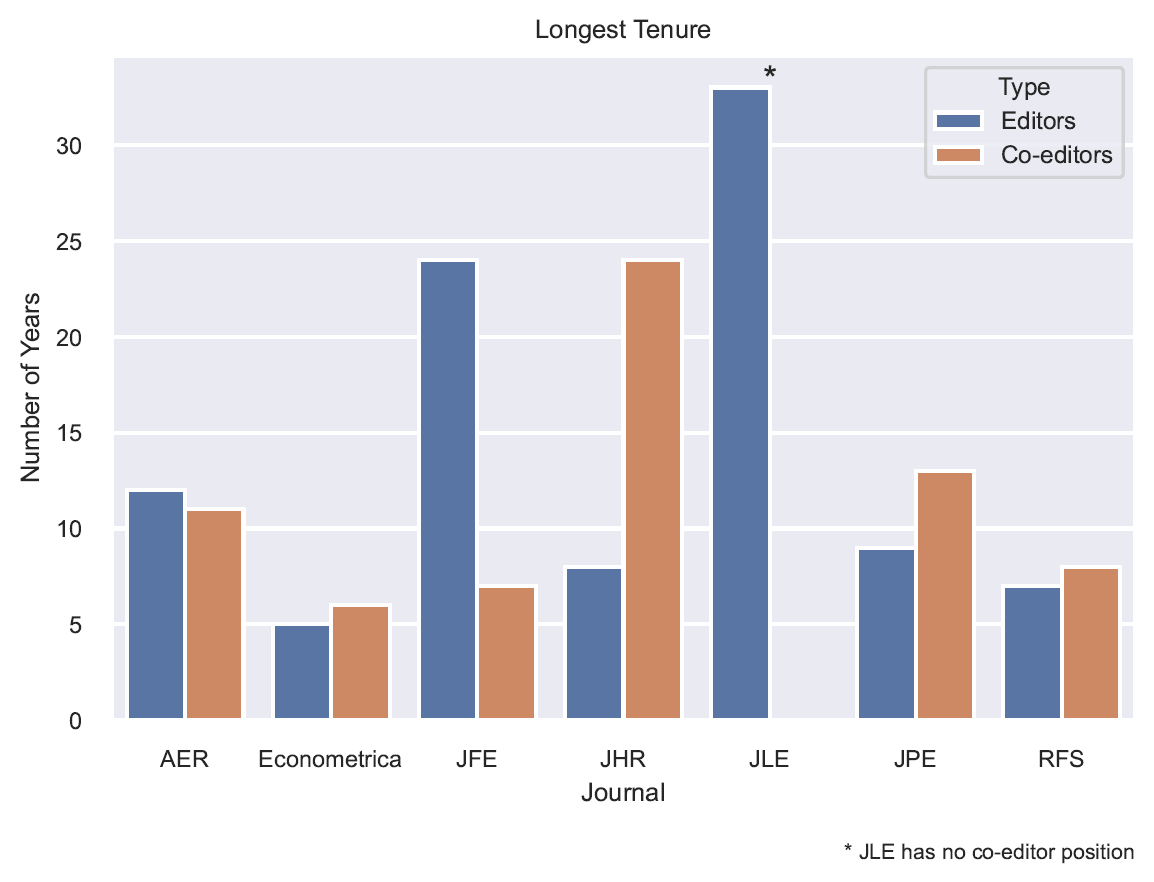
\includegraphics[width=\textwidth]{figures/editors_max_tenure.png}
    \caption{Results of the Scopus-EconLit Matching Process}
\end{figure}


\begin{figure}[h]
    \centering
    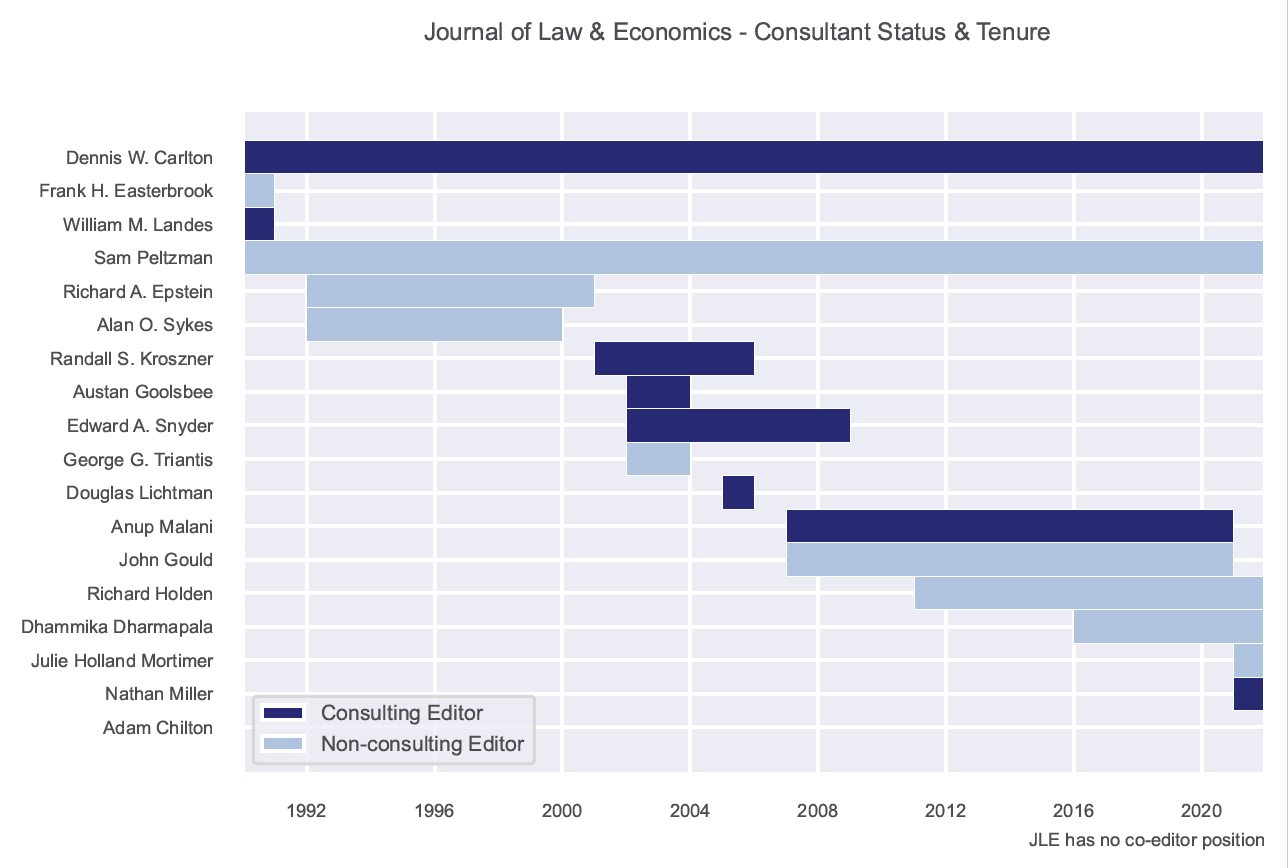
\includegraphics[width=\textwidth]{figures/editors_jle_history.png}
    \caption{Editorial Composition of the \textit{Journal of Law and Economics} (1990-2020)}
\end{figure}
\begin{figure}[h]
    \centering
    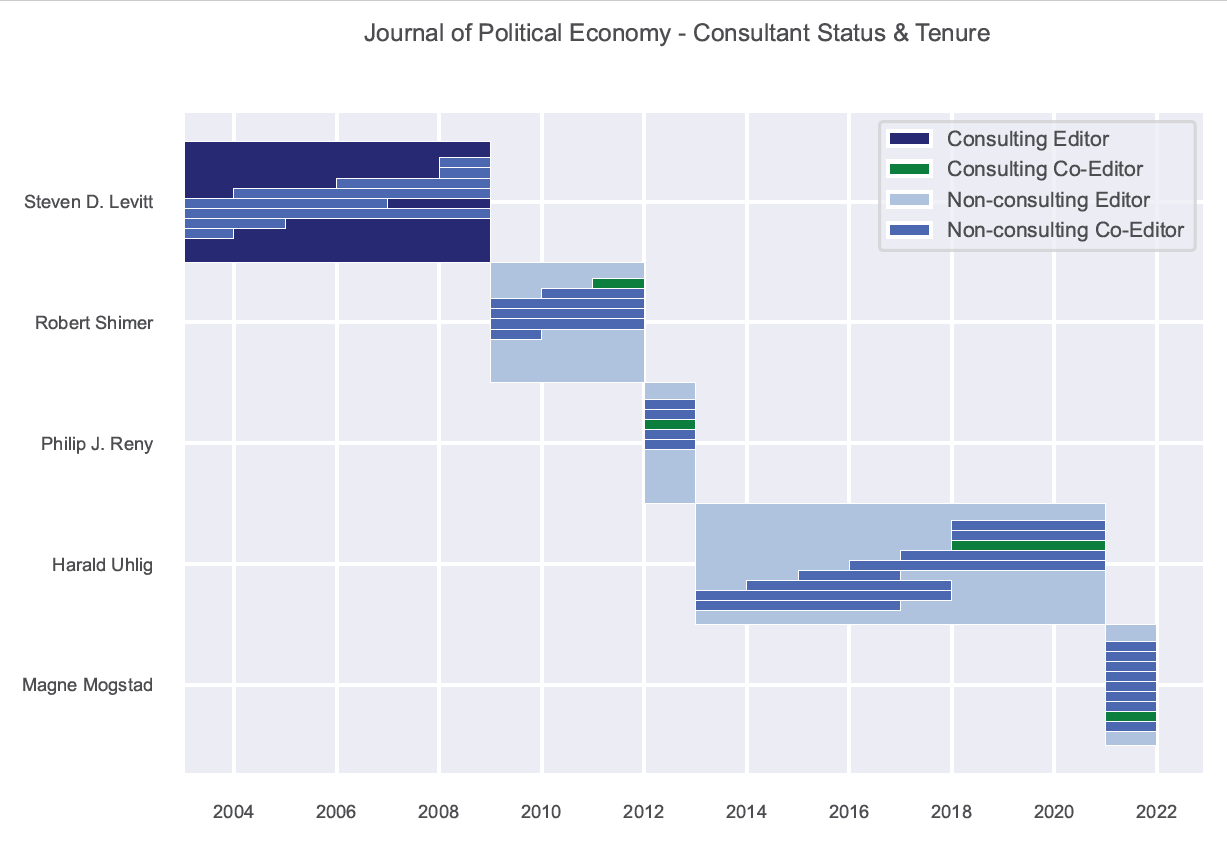
\includegraphics[width=\textwidth]{figures/editors_jpe_history.png}
    \caption{Editorial Composition of the \textit{Journal of Political Economy} (2002-2020)}
\end{figure}








    
\appendix
\section{Author Rankings, by journal}


\newpage
\begin{landscape}
    \thispagestyle{empty}
        
% Table created by stargazer v.5.2.3 by Marek Hlavac, Social Policy Institute. E-mail: marek.hlavac at gmail.com
% Date and time: Wed, Jul 27, 2022 - 9:52:29 PM
\begin{table}[!htbp] \centering 
  \caption{Most Published Authors (Top 5)} 
  \label{} 
\footnotesize 
\begin{tabular}{@{\extracolsep{5pt}} l<{\raggedright}p{0.17\linewidth}<{\raggedright}p{0.17\linewidth}<{\raggedright}p{0.17\linewidth}<{\raggedright}p{0.17\linewidth}<{\raggedright}p{0.17\linewidth}<{\raggedright}p{0.17\linewidth}} 
\\[-1.8ex]\hline 
\hline \\[-1.8ex] 
Rank & AER & ECA & JPE & QJE & RES \\ 
\hline \\[-1.8ex] 
1 & John J. Siegfried (42) & Donald W.K. Andrews (24) & Daron Acemoglu (19) & Andrei Shleifer (18) & Daron Acemoglu (11) \\ 
2 & Daron Acemoglu (29) & Whitney Newey (19), Peter C.B. Phillips (19) & Pierre Andre Chiappori (11) & Emmanuel Saez (14) & Jean Tirole (10) \\ 
3 & John A. List (21) & Matthew O. Jackson (13) & James J. Heckman (10) & Sendhil Mullainathan (13), Daron Acemoglu (13) & Emmanuel Farhi (9), Richard Blundell (9) \\ 
4 & Peter L. Rousseau (20), Ernst Fehr (20) & Victor Chernozhukov (12) & Jean Tirole (9), John A. List (9) & Raj Chetty (12) & Costas Meghir (8), Bruno Biais (8), Patrick Bolton$^{\mathsection}$ (8) \\ 
5 & By Esther Duflo (19), Jean Tirole (19) & Guido W. Imbens (11), Larry Samuelson (11) & Sergio Rebelo (8), Kevin M. Murphy (8) & Michael Kremer (11) & Philippe Aghion (7), Debraj Ray (7), Matthew O. Jackson (7), Martin Browning (7) \\ 
6 & David Autor (18), Alvin E. Roth (18), Alan J. Auerbach (18) & Elie Tamer (10), Massimo Marinacci (10), Joel L. Horowitz (10), Jinyong Hahn (10), Ulrich K. Muller (10), Xiaohong Chen (10) & Andrei Shleifer (7) & Timothy Besley (10), David Card (10), Marianne Bertrand (10), Jeremy C. Stein$^{\mathsection}$ (10) & \\ 
7 & & & Martin Eichenbaum (6), Michael Greenstone (6), Boyan Jovanovic (6), Patrick J. Kehoe (6), Mark Rosenzweig (6), Gene M. Grossman (6), Abhijit Banerjee (6) & & \\ 
8 & & & & & \\ 
\hline \\[-1.8ex] 
\multicolumn{6}{l}{\footnotesize{$^{\dag}$: Law and Economics; $^{*}$: Industrial Organization; $^{\dag}$: Labor Studies; $^{\mathsection}$: Corporate Finance.}} \\ 
\end{tabular} 
\end{table} 

\end{landscape}
\newpage
\begin{landscape}
    \thispagestyle{empty}
        
% Table created by stargazer v.5.2.3 by Marek Hlavac, Social Policy Institute. E-mail: marek.hlavac at gmail.com
% Date and time: Wed, Jul 27, 2022 - 9:52:34 PM
\begin{table}[!htbp] \centering 
  \caption{Most Published Authors (Finance and Labor)} 
  \label{} 
\footnotesize 
\begin{tabular}{@{\extracolsep{5pt}} ccccc} 
\\[-1.8ex]\hline 
\hline \\[-1.8ex] 
Rank & JOF & JFE & RFS & JOL \\ 
\hline \\[-1.8ex] 
1 & Sheridan Titman\textbackslash mathsection (26) & Rene M. Stulz\textbackslash mathsection (35) & Rene M. Stulz\textbackslash mathsection (19) & David CardNA (11) \\ 
2 & Andrei ShleiferNA (20) & G. William SchwertNA (32) & Viral AcharyaNA (16) & Edward P. LazearNA (9) \\ 
3 & Francis A. LongstaffNA (18) & Jerold B. WarnerNA (28) & Matthew SpiegelNA (14) & c("Kenneth R. TroskeNA (8)", "Kathryn ShawNA (8)", "Peter KuhnNA (8)", "David NeumarkNA (8)") \\ 
4 & Jeremy C. Stein\textbackslash mathsection (16) & Clifford W. SmithNA (27) & c("Maureen O'HaraNA (13)", "Massimo MassaNA (13)", "John M. GriffinNA (13)") & c("Todd StinebricknerNA (6)", "James J. HeckmanNA (6)", "Yoram WeissNA (6)", "Michael BakerNA (6)") \\ 
5 & c("Maureen O'HaraNA (15)", "Paul SchultzNA (15)", "Campbell R. HarveyNA (15)") & Richard S. RubackNA (26) & David Hirshleifer\textbackslash mathsection (11) & NULL \\ 
6 & c("Eugene F. FamaNA (14)", "Rene M. Stulz\textbackslash \textbackslash mathsection (14)", "Kenneth R. FrenchNA (14)", "Raghuram RajanNA (14)") & Michael C. Jensen\textbackslash mathsection (25) & c("Thierry FoucaultNA (10)", "Roni MichaelyNA (10)", "Avanidhar SubrahmanyamNA (10)") & NULL \\ 
7 & NULL & John B. LongNA (24) & NULL & NULL \\ 
8 & NULL & c("Wayne H. MikkelsonNA (19)", "Andrei ShleiferNA (19)", "Avanidhar SubrahmanyamNA (19)") & NULL & NULL \\ 
\hline \\[-1.8ex] 
\multicolumn{5}{l}{Symbols indicate being a consultant and affiiated with an NBER program: $^{\dag}$: Law and Economics; $^{*}$: Industrial Organization; $^{\dag}$: Labor Studies; $^{\mathsection}$: Corporate Finance.} \\ 
\end{tabular} 
\end{table} 

\end{landscape}
\newpage
\begin{landscape}
    \thispagestyle{empty}
    
% Table created by stargazer v.5.2.3 by Marek Hlavac, Social Policy Institute. E-mail: marek.hlavac at gmail.com
% Date and time: Wed, Jul 27, 2022 - 4:52:31 PM
\begin{table}[!htbp] \centering 
  \caption{Most Published Authors (IO \& Law and Economics)} 
  \label{} 
\begin{adjustbox}{max width = \textwidth}
\scriptsize 
\begin{tabular}{@{\extracolsep{5pt}} l<{\raggedright}p{0.12\linewidth}<{\raggedright}p{0.12\linewidth}<{\raggedright}p{0.12\linewidth}<{\raggedright}p{0.12\linewidth}<{\raggedright}p{0.12\linewidth}<{\raggedright}p{0.12\linewidth}<{\raggedright}p{0.12\linewidth}<{\raggedright}p{0.12\linewidth}} 
\\[-1.8ex]\hline 
\hline \\[-1.8ex] 
Rank & ATB & ALJ & JEM & JHR & JLE & JLO & RJE \\ 
\hline \\[-1.8ex] 
1 & Roger D. Blair (25) & Jonathan B. Baker (14) & Daniel F. Spulber (10) & David Neumark (13) & Eric Helland (8) & Pablo T. Spiller$^{\dag}$ (11) & Jean Tirole (16) \\ 
2 & Gregory T. Gundlach (16) & William E. Kovacic (12), Gregory J. Werden (12) & David P. Baron (8) & Janet Currie (9) & Thomas Stratmann (7), Dennis W. Carlton$^{\textasteriskcentered }$ (7) & Jennifer F. Reinganum (10) & Jennifer F. Reinganum (12) \\ 
3 & Albert A. Foer (13) & Steven C. Salop (11) & David E.M. Sappington (7) & James P. Smith (7) & Tomas J. Philipson (6) & Andrew F. Daughety (9) & Andrew F. Daughety (11), David Martimort (11) \\ 
4 & William E. Kovacic (10), Diana L. Moss (10) & Timothy J. Muris (10) & Ramon Casadesus-Masanell (6), Esther Gal-Or (6), Stuart J.H. Graham (6) & James J. Heckman (6), Duncan Thomas (6) & F. Andrew Hanssen (5), Sam Peltzman (5), John R. Lott (5), Anup Agrawal (5), Peter T. Leeson (5), Joseph J. Sabia (5), Benjamin Klein (5) & Abraham L. Wickelgren (8) & Roman Inderst (10), Yongmin Chen (10) \\ 
5 & John E. Kwoka (9), Mark A. Glick (9) & Benjamin Klein (9) & Konstantinos Serfes (5), Robert Fairlie (5), Alan C. Marco (5), Luis M.B. Cabral (5), Juan Jose Ganuza (5) & Joseph G. Altonji (5), James P. Ziliak (5), Heather Antecol (5), Hilary Hoynes (5), Thomas DeLeire (5), Robert Moffitt (5), Steven G. Rivkin (5), Audrey Light (5), Steven Haider (5), Bruce D. Meyer (5), D. M. Blau (5), Philip Oreopoulos (5) & & Benjamin E. Hermalin (7) & Kathryn E. Spier (9), Benjamin E. Hermalin (9), Bruno Jullien (9), Gary Biglaiser (9), Greg Shaffer (9), Patrick Rey (9) \\ 
6 & Malcolm B. Coate (8), Daniel J. Gifford (8), Sumit K. Majumdar (8), John E. Lopatka (8), Charles D. Weller (8) & Warren S. Grimes (7), Carl Shapiro$^{\textasteriskcentered }$ (7), Eleanor M. Fox (7) & & & & Steven Shavell$^{\dag}$ (6), Alan Schwartz (6) & \\ 
7 & & Willard K. Tom (6), Douglas H. Ginsburg (6), Marc Winerman (6), William H. Page (6), Daniel A. Crane (6), Joshua D. Wright (6) & & & & Emerson H. Tiller (5), Barry R. Weingast (5), Nuno Garoupa (5), Stephen J. Choi (5), Eric L. Talley (5), Ricard Gil (5), David Epstein (5) & \\ 
8 & & & & & & & \\ 
\hline \\[-1.8ex] 
\end{tabular} 
\end{adjustbox} 
\end{table} 

\end{landscape}
    



\end{document}